\documentclass[border=2pt]{standalone}
\usepackage{helvet}\renewcommand{\familydefault}{\sfdefault}
\usepackage{tikz}
\usetikzlibrary{arrows.meta, positioning, fit, backgrounds, calc}
\begin{document}
\linespread{1}\selectfont
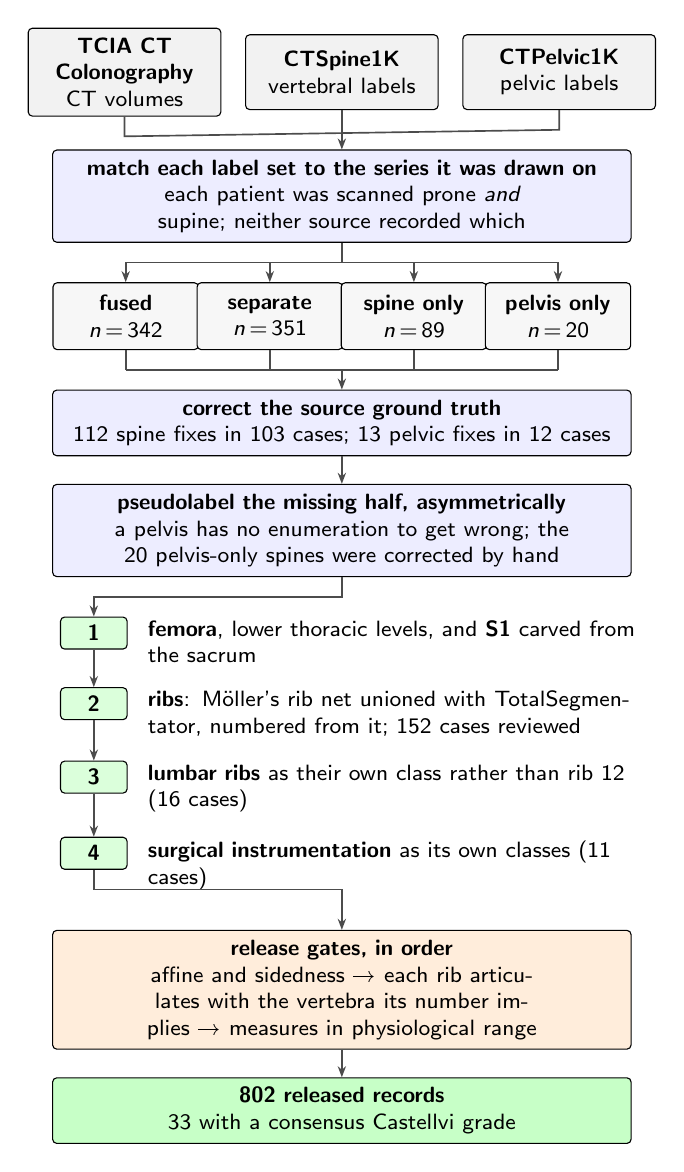
\begin{tikzpicture}[
  % absolute 8 pt: the boxes are sized in millimetres, so the type must not follow the
  % document size (\footnotesize is 10 pt in the preprint and wrapped every box)
  x=1mm, y=1mm, font=\sffamily\fontsize{8}{9.6}\selectfont, node distance=3.5mm,
  bx/.style={draw, rounded corners=1.5pt, align=center, text width=#1, inner sep=3.5pt},
  src/.style={bx=22mm, fill=black!5, minimum height=9.5mm},
  proc/.style={bx=71mm, fill=blue!7},
  rec/.style={bx=16mm, fill=black!3, minimum height=8.5mm},
  ver/.style={bx=6mm, fill=green!14, inner ysep=3pt},
  det/.style={align=left, text width=62mm, inner sep=0pt},
  gate/.style={bx=71mm, fill=orange!14},
  fin/.style={bx=71mm, fill=green!22},
  ar/.style={-{Stealth[length=4pt]}, semithick, black!70},
  ln/.style={semithick, black!70},
]
% sources
\node[src] (spine) at (0, 0) {\textbf{CTSpine1K}\\vertebral labels};
\node[src, left=3mm of spine]  (tcia)   {\textbf{TCIA CT Colonography}\\CT volumes};
\node[src, right=3mm of spine] (pelvic) {\textbf{CTPelvic1K}\\pelvic labels};
\node[proc, below=5mm of spine] (cross) {\textbf{match each label set to the series it was drawn on}\\
  each patient was scanned prone \emph{and} supine; neither source recorded which};
\draw[ln] (tcia.south) -- ($(tcia.south)+(0,-2.5mm)$) -- ($(pelvic.south)+(0,-2.5mm)$) -- (pelvic.south);
\draw[ar] (spine.south) -- (cross.north);
% record types, on a bus
\node[rec, anchor=north] (fused) at ($(cross.south)+(-27.45mm,-5mm)$) {\textbf{fused}\\\textit{n}\,=\,342};
\node[rec, anchor=north] (sep)   at ($(cross.south)+(-9.15mm,-5mm)$)  {\textbf{separate}\\\textit{n}\,=\,351};
\node[rec, anchor=north] (sonly) at ($(cross.south)+(9.15mm,-5mm)$)   {\mbox{\textbf{spine only}}\\\textit{n}\,=\,89};
\node[rec, anchor=north] (ponly) at ($(cross.south)+(27.45mm,-5mm)$)  {\mbox{\textbf{pelvis only}}\\\textit{n}\,=\,20};
\draw[ln] (cross.south) -- ($(cross.south)+(0,-2.5mm)$);
\draw[ln] ($(fused.north)+(0,2.5mm)$) -- ($(ponly.north)+(0,2.5mm)$);
\foreach \n in {fused,sep,sonly,ponly} \draw[ar] ($(\n.north)+(0,2.5mm)$) -- (\n.north);
% corrections and pseudolabels
\node[proc, anchor=north] (fix) at ($(cross.south |- fused.south)+(0,-5mm)$) {\textbf{correct the source ground truth}\\
  112 spine fixes in 103 cases; 13 pelvic fixes in 12 cases};
\foreach \n in {fused,sep,sonly,ponly} \draw[ln] (\n.south) -- ($(\n.south)+(0,-2.5mm)$);
\draw[ln] ($(fused.south)+(0,-2.5mm)$) -- ($(ponly.south)+(0,-2.5mm)$);
\draw[ar] ($(fix.north)+(0,2.5mm)$) -- (fix.north);
\node[proc, below=of fix] (dense) {\textbf{pseudolabel the missing half, asymmetrically}\\
  a pelvis has no enumeration to get wrong; the 20 pelvis-only spines were corrected by hand};
\draw[ar] (fix.south) -- (dense.north);
% versions
\node[ver, anchor=north west] (v3) at ($(dense.south west)+(1mm,-5mm)$) {\textbf{1}};
\node[det, anchor=north west] (d3) at ($(v3.north east)+(2.5mm,-0.5mm)$) {\textbf{femora}, lower thoracic levels, and \textbf{S1} carved from the sacrum};
\node[ver, anchor=north west] (v4) at ($(v3.south west |- d3.south)+(0,-3mm)$) {\textbf{2}};
\node[det, anchor=north west] (d4) at ($(v4.north east)+(2.5mm,-0.5mm)$) {\textbf{ribs}: M\"oller's rib net unioned with TotalSegmentator, numbered from it; 152 cases reviewed};
\node[ver, anchor=north west] (v5) at ($(v4.south west |- d4.south)+(0,-3mm)$) {\textbf{3}};
\node[det, anchor=north west] (d5) at ($(v5.north east)+(2.5mm,-0.5mm)$) {\textbf{lumbar ribs} as their own class rather than rib~12 (16 cases)};
\node[ver, anchor=north west] (v6) at ($(v5.south west |- d5.south)+(0,-3mm)$) {\textbf{4}};
\node[det, anchor=north west] (d6) at ($(v6.north east)+(2.5mm,-0.5mm)$) {\textbf{surgical instrumentation} as its own classes (11 cases)};
\draw[ar] (dense.south) -- ($(dense.south)+(0,-2.5mm)$) -| (v3.north);
\draw[ar] (v3.south) -- (v4.north); \draw[ar] (v4.south) -- (v5.north); \draw[ar] (v5.south) -- (v6.north);
% gates and release
\node[gate, anchor=north] (qc) at ($(dense.south |- d6.south)+(0,-5mm)$) {\textbf{release gates, in order}\\
  affine and sidedness \textrightarrow\ each rib articulates with the vertebra its number implies
  \textrightarrow\ measures in physiological range};
\draw[ar] (v6.south) -- ($(v6.south)+(0,-2.5mm)$) -| (qc.north);
\node[fin, below=of qc] (rel) {\textbf{802 released records}\\33 with a consensus Castellvi grade};
\draw[ar] (qc.south) -- (rel.north);
\end{tikzpicture}
\end{document}
